\documentclass[10pt]{article}
\usepackage{amsmath, amssymb, amsfonts}
\usepackage{amsthm}
\usepackage{geometry} % For 1 inch margins
\usepackage{graphicx} % For including images
\usepackage{times} % For Times New Roman font
\usepackage{lipsum} % For generating dummy text
\usepackage[utf8]{inputenc} % For UTF-8 encoding
\usepackage{titlesec} % For customizing titles
\usepackage{titling} % For customizing the title
\usepackage{fancyhdr} % For custom headers and footers
\usepackage{tikz}
\usepackage{slashed}
\usepackage{everypage}
\usepackage{titlesec}
\usepackage{ulem} % Needed for underlining
\usepackage{multicol}

\usepackage{tikz}

\usetikzlibrary{graphs}
\usetikzlibrary{shapes}
\usetikzlibrary{backgrounds}
\usetikzlibrary{calc}
\usetikzlibrary{patterns}
\usetikzlibrary{positioning, fit, arrows.meta}

\setlength{\leftskip}{2em}
\geometry{
    textheight=9in,
    textwidth=5.5in,
    top=1in,
    headheight=12pt,
    headsep=12.5pt,
    footskip=30pt
}

\newenvironment{solution}{\textit{Solution}.}

\newcommand{\proofseparator}{\noindent\makebox[\linewidth]{\rule{\textwidth}{0.4pt}}}

\newcommand{\sol}[1]{
    \vspace{5pt}
    \begin{solution}
    #1
    \end{solution}
    \proofseparator
}

% Natural Numbers 
\newcommand{\N}{\ensuremath{\mathbb{N}}}

% Whole Numbers
\newcommand{\W}{\ensuremath{\mathbb{W}}}

% Integers
\newcommand{\Z}{\ensuremath{\mathbb{Z}}}

% Rational Numbers
\newcommand{\Q}{\ensuremath{\mathbb{Q}}}

% Real Numbers
\newcommand{\R}{\ensuremath{\mathbb{R}}}

% Complex Numbers
\newcommand{\C}{\ensuremath{\mathbb{C}}}


\pagestyle{fancy}
\fancyhf{} % Clear default header and footer settings
\fancyhead[L]{TAKE HOME EXAM 2} % Custom left header
\fancyhead[R]{Paul Beggs} % Custom right header
\rfoot{Page \thepage} % Right footer with the page number

\begin{document}
\newpage

\begin{enumerate}
    \setcounter{enumi}{1}
    \item Suppose that $f\colon X\rightarrow Y$ is a one-to-one and onto function.

          \begin{enumerate}
              \vspace{0.5cm}

              \item Briefly, explain how you know $f^{-1} \colon Y \rightarrow X$ is a function which indeed uses all of $Y$ as its domain. \\

                    \sol{
                        \dots $Y\rightarrow X$, then by definition, it too, must map each $x$ to $y$ by definition. Hence, each $y$ in the domain is mapped to a unique $x$ is in the co-domain.
                    }

                    \vspace{0.5cm}

              \item Show that $f^{-1}$ is one-to-one. \\

                    \sol{
                        Let $f\colon X \rightarrow Y$ be a one-to-one and onto function. Also let $f^{-1}$ be the inverse function of $f$, defined as $f^{-1} \colon Y \rightarrow X$. \\

                        To prove that $f^{-1}$ is one-to-one, we must show that if $f^{-1}(y_1) = f^{-1}(y_2)$ for any $y_1,y_2 \in Y$, then $y_1 = y_2$. \\

                        Assume $y_1,y_2 \in Y$ and that $f^{-1}(y_1) = f^{-1}(y_2)$. Because of the definition of the inverse function, since  $f^{-1}(y_1) = x_1$ and $f^{-1}(y_2) = x_2$, then $f(x_1) = y_1$ and $f(x_2) = y_2$ which implies $x_1 = x_2$ by substitution. Since, $f(x_1) = y_1$ and $f(x_2) = y_2$, and given that $f$ is one-to-one, it follows that $y_1 = y_2$.
                    }

                    \vspace{0.5cm}

              \item Show that $f^{-1}$ is onto. \\

                    \sol{
                        Let $f\colon X \rightarrow Y$ be a one-to-one and onto function. Also let $f^{-1}$ be the inverse function of $f$, defined as $f^{-1} \colon Y \rightarrow X$. \\

                        To prove that $f^{-1}$ is onto, we must show that for every element $x\in X$, there exists an element $y\in Y$ such that $f^{-1}(y) = x$. \\

                        Let any $x\in X$. Since $f$ is onto, there exists a $y\in Y$ such that $f(x) = y$. Then, by the definition of the inverse function, if $f(x) = y$ then $f^{-1}(y) = x$. Thus, $f^{-1}$ is onto.
                    }
          \end{enumerate}

          \vspace{0.3cm}

    \item Construct a function $f \colon \Z \rightarrow \N$ which is onto, but is not one-to-one. Justify your answer. \\

          \sol{
              Consider the piece-wise function (where $z\in \Z)$,
              $f(z) =
                  \begin{cases}
                      -z    & \text{if } z < 0,   \\
                      z + 1 & \text{if } z \geq 0
                  \end{cases} $ \\

              This function is onto because for every natural number $n\in \N$ in the co-domain, there exists at least one element in the domain, $z\in \Z$, that maps to it. In other words, if $n > 0$, then $f(-n) = n$ (for negative numbers), and $f(n-1) = n$ (for non-negative inputs). Thus, at least one integer maps to every natural number. \\

              However, this function is not one-to-one because for any $n > 0$, there are two $z\in \Z$ such that $z_1 = -(n)$ and $z_2 = n - 1$ such that $f(z_1) = n$ and $f(z_2) = n$
          }

          \newpage

    \item Construct a function $g\colon \N \rightarrow \N$ which is one-to-one, but not onto. Justify your answer. \\

          \sol{
              Consider $g(n) = n + 1$ (where $n\in \N$). \\

              This function is one-to-one because for every $n\in N$, $g(n)$ maps to $n + 1$. By definition, this mapping is one-to-one because for every $n_1,n_2 \in N$, if $g(n_1) = g(n_2)$, then $n_1 + 1 = n_2 + 1$, which simplifies to $n_1 = n_2$. \\

              It is not onto because there does not exist an $n\in N$ for which $g(n) = 1$. In other words, $1$ (in the co-domain) is never mapped to by an element in the domain.
          }

          \vspace{0.3cm}

    \item Find a function $h \colon \N \rightarrow \Z$ which is \textit{both} one-to-one and onto. Justify your answer. \\

          \sol{
              Consider the piece-wise function (where $n\in \N$),
              $h(n) =
                  \begin{cases}
                      \frac{n}{2}      & \text{if } n \text{ is even}, \\
                      -\frac{n + 1}{2} & \text{if } n \text{ is odd}
                  \end{cases} $ \\

              For even $n\in \N$, $h(n)$ produces a non-negative integer\footnote{Why do we always say `non-negative' and not `positive?'}, and for odd $n$, it produces a negative integer. The really cool thing about this, is that for each corresponding mapping, if $n$ is even, $h(n)$ produces a non-negative integer, and if $n$ is odd, $h(n)$ produces a negative integer. This ensures that each $n$ maps to a unique $z\in \Z$. Thus, $h(n)$ is one-to-one. \\

              For every integer $z\in \Z$, there exists a natural number $n\in \N$ such that $h(n) = z$. Furthermore, if $z\geq 0$, we can take $n = 2z$, which is an even natural number that maps to $z$ (by the definition of even numbers). Conversely, if $z < 0$, we can take $n = -2z - 1$, which is an odd natural number that maps to $z$ (by the definition of odd numbers). Thus, this ensures that every integer is the image of some natural number. Thus, $h(n)$ is onto.
          }

          \vspace{0.3cm}

    \item Suppose that $R$ is an equivalence relation on $X$ and let $a,b \in X$ so that $a\ \slashed{R} \ b$, that is, $a$ is not related to $b$. Show that $$[a] \cap [b] = \emptyset$$

          \textbf{Goal}: Prove that if $a$ and $b$ are not related by $R$, then their equivalence classes have no elements in common. In other words, the intersection of the two equivalence classes has no elements. \\

          \sol{
              For the sake of contradiction, suppose that $[a] \cap [b] \ne \emptyset$. By the denial of the empty set, this means there must exist an element $c\in X$ such that $c\in [a]$ and $c\in [b]$. Then, by the definition of equivalence classes, this means that $c  \ R \  a$, and $c  \ R \  b$ . Given these relations, by respectively using symmetry and transitivity, we can show that since $c  \ R \  a$, then $a  \ R \  c$, and because $a  \ R \  c$ and $c  \ R \  b$, then $a  \ R \  b$. \\

              However, $a  \ R \  b$ contradicts the given information, so our assumption must be false. Hence, it must be the case that $[a]\cap [b] = \emptyset$.
          }

          \newpage

          For the following problem, define $R\colon V \rightarrow V$ by $a \ R \  b \iff b$ is a path connected to $a$:

    \item Suppose $G = (V,E)$ is a simple graph, which might not be connected. Let $v \in V$. For each vertex $u\in V$, we say that $v$ is a \textit{path connected} to $u$ provided that there exists a path from $v$ to $u$. Is $R$ an equivalence relation? [Hint: $R$ is reflexive, since any vertex $v$ is path connected to itself by the simple path: $v$.] \\

          \sol{
              Let $u,v\in V$ with $R\colon V \rightarrow V$ by $a \ R \  b$ if, and only if, $b$ is a path connected to $a$. To show that $R$ is an equivalence relation, we need to show three things:
              \begin{enumerate}
                  \item \textbf{Reflexivity}: \\
                        For $R$ to be reflexive, every vertex $v\in V$ must be a path connected to itself. This is proven true by the hint provided.
                  \item \textbf{Symmetry}:  \\
                        For $R$ to be symmetric, if $v  \ R \  u$ (indicative of a path connected from $v$ to $u$), then $u  \ R \  v$ (path connected from $u$ to $v$ by definition). Because the given information does not specify that $G$ or the relation $a  \ R \  b$ is a \textit{directed graph}, one can assume that this \textit{path connected} is non-directed, and hence, is intrinsically symmetric because the of the non-directional nature of the graph or path. In other words, if $v  \ R \  u$, then $u  \ R \  v$ and vice versa because it does not matter at which vertex you begin at (in this context).
                  \item \textbf{Transitivity}: \\
                        For $R$ to be transitive, if $v  \ R \  u$, and $u  \ R \  w$, then $v  \ R \  w$. Because the vertices $v,u$ and $u,w$ are path connected, there exists edges that connect these vertices together to form a path. Hence, because there is a path that stretches from $v$ to $w$, then $v  \ R \  w$. \\
              \end{enumerate}
          }

          \vspace{0.3cm}

    \item Draw two trees with 5 vertices which are not isomorphic. Explain how you know they are not isomorphic.


          \begin{multicols}{2}
              \centering
              \noindent

              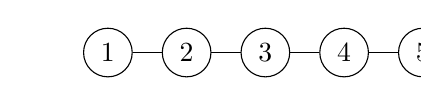
\begin{tikzpicture}[every node/.style={draw,circle}]
                  \node (a) at (0,0) {1};
                  \node (b) at (1,0) {2};
                  \node (c) at (2,0) {3};
                  \node (d) at (3,0) {4};
                  \node (e) at (4,0) {5};
                  \draw (a) -- (b) -- (c) -- (d) -- (e);
              \end{tikzpicture} \\

              Graph $G$

              \columnbreak

              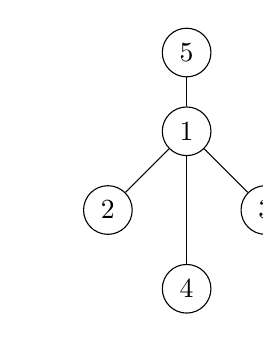
\begin{tikzpicture}[every node/.style={draw,circle}]
                  \node (a) at (2,2) {1};
                  \node (b) at (1,1) {2};
                  \node (c) at (3,1) {3};
                  \node (d) at (2,0) {4};
                  \node (e) at (2,3) {5};
                  \draw (a) -- (b);
                  \draw (a) -- (c);
                  \draw (a) -- (d);
                  \draw (a) -- (e);
              \end{tikzpicture} \\

              Graph $H$

          \end{multicols}

          \sol{
              Let $G = (V,E)$ and $H = (W,F)$ (with $V,W$ being the vertex sets, and $E,F$ being the edge sets). Then, \\

              $G = \{\{1,2,3,4,5\}, \{\{1,2\},\{2,3\},\{3,4\},\{4,5\}\}\}$ and \\
              $F = \{\{1,2,3,4,5\}, \{\{1,2\},\{1,3\},\{1,4\},\{1,5\}\}\}$. \\

              For $G$ to be \textit{isomorphic} to $H$, the process must preserve the degrees of corresponding vertices. Since $G$ has vertices degrees of 1, 2, 2, 2, and 1 for vertices 1-5 and $H$ has vertices 2-5 with $\deg(1)$, and vertex 1 with $\deg(4)$ these graphs are not bijective.
          }

          \newpage

    \item Suppose that $T$ is a tree. Show that $T$ must contain at least two vertices of odd degree.

          \sol{
              Suppose $T$ is a tree. By the Handshake Theorem, we know that the sum of the degrees of $T$'s vertices is always twice the sum of the edges. So, $\Sigma \deg(v) = 2E$ (where $E$ is the set of edges). Then, we know that by Theorem 1, a tree with $n$ vertices, has $n-1$ edges. So, we can rewrite the equation to be $\Sigma \deg(v) = 2(n - 1)$. \\

              Now, assume for the sake of contradiction that $T$ has fewer than two vertices of odd degree. Then, there are two possible cases for $T$'s vertices' degree. Either:
              \begin{enumerate}
                  \item No vertices of odd degree, or
                  \item exactly one vertex of odd degree.
              \end{enumerate}
              We know that the first case must be false because the lemma to Theorem 1 says that, ``If $G$ is a tree, $G$ has at least one vertex of degree 1.'' \\
              And well, we know that it cannot be the second case because Corollary 2 to the Handshake Theorem says that no graph can have exactly one vertex of odd degree. \\

              Therefore, it must be the case that our assumption was false, and $T$ must have an even number of vertices with an odd degree. And as shown, since $T$ cannot have no vertices of odd degree (0), and 1 is odd, then the minimum number of even vertices with odd degree $T$ can have is 2.
          }
\end{enumerate}
\end{document}